\chapter{Seiyuu Social Network}
Social networks consist of a finite set of actors and the relations between them. Usually represented as a graph; with actors or organizations as set of nodes and a defined relation between them as set of edges. This structures are useful to analyze complex social interactions and communities.

\section{Node and edge definition}
Our social network consists of voice actors (seiyuu) as nodes and co-workership between them as edges. It's important to notice that this social network is time dependant since each seiyuu has a debut year and each anime has an aired time; giving us freedom to choose different time frames to observe.

Aside from being time dependant there exists different possible definitions of relationship or co-workership between seiyuu. One could say two actors know each other if they have worked in at least one job together, or maybe it requires more than one. There's also a time frame to define, relationship could take into account all works of both of them or only from certain years.

TODO EXPLICAR EL HECHO DE QUE ES UNA TWO MODE NETWORK Y DESPUES PONER QUE ELEGIMOS USAR SEIYUU COMO NODOS PERO PODRIA SER AL REVES

TODO MOVER EL SIGUIENTE PARRAFO AL FINAL DE ESTE CAPITULO
After observing graphs built with different interpretations of relationship, the criteria for connecting two nodes became: \textit{at least 10 works in common, during the time frame between the first debut registered (1960) and the year of observation}.
Because requiring more jobs in common means less amount of edges, this leaves a more understandable graph and we verified it does without changing its structure.

There's also other interesting definitions of relationship, for example we can use only common works from the last x years or from all time. This options weren't explored; having into account our limited time we opted to decide on TODO PARAFRASEAR ESTO UN POCO MAS one that was more useful or logic and put more effort in analyzing the data and social network at hand.

\section{Construction}
As a first approach Gephi was used to build the network. Since the graph was big enough to bring performance problems and we needed to build the edges dynamically (which couldn't be done in Gephi) NetworkX was used instead.

NetworkX was chosen because it's an easy yet powerful Python library, it doesn't get along with massive graphs but ours was not big enough to present a problem. One can also export the graph and open it on Gephi, for a more visual analysis.

We needed to build the edges dynamically because they depend on the time frame we are looking at. For example if two actors worked together in 9 jobs between 1960 and 1970 we shouldn't see an edge between them; but if they worked together again in 1971 then looking at 1960-1971 they should be connected.

\section{Analysis}
Is easy to tell at first glance that this social network is really interconnected. With only 2956 nodes it has 395887 edges when only one work in common is required and 13629 edges when asking for 10 or more. It shows a thightly interconnected cluster surrounded by poorly or not connected nodes. This cluster represents 99\% of the nodes of one work in common graph and 23\% of 10 works in common. In terms of modularity we can see at least four clear communities in each graph, Fig~\ref{fig:graph1CommunityColoured} and Fig~\ref{fig:graph10CommunityColoured}.

\begin{figure}[!hbt]
	\begin{center}
	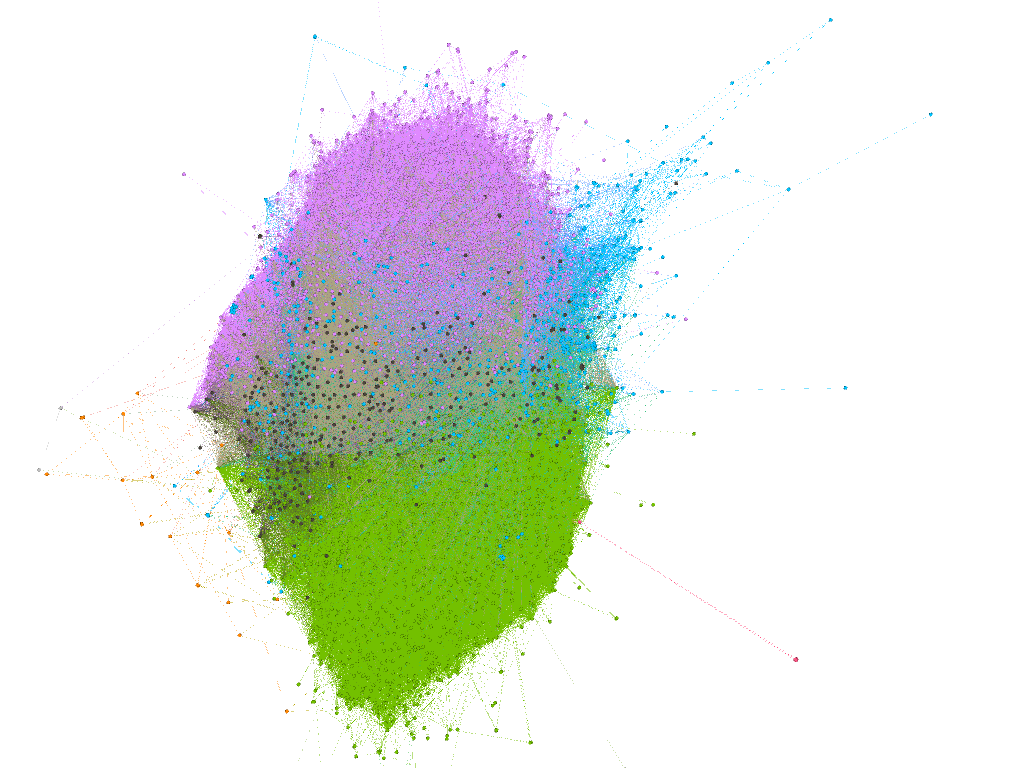
\includegraphics[width=\columnwidth]{graphics/atLeast1WorkCommunity.png}
	\caption{At least one work in common graph coloured by community.}
	\label{fig:graph1CommunityColoured}

	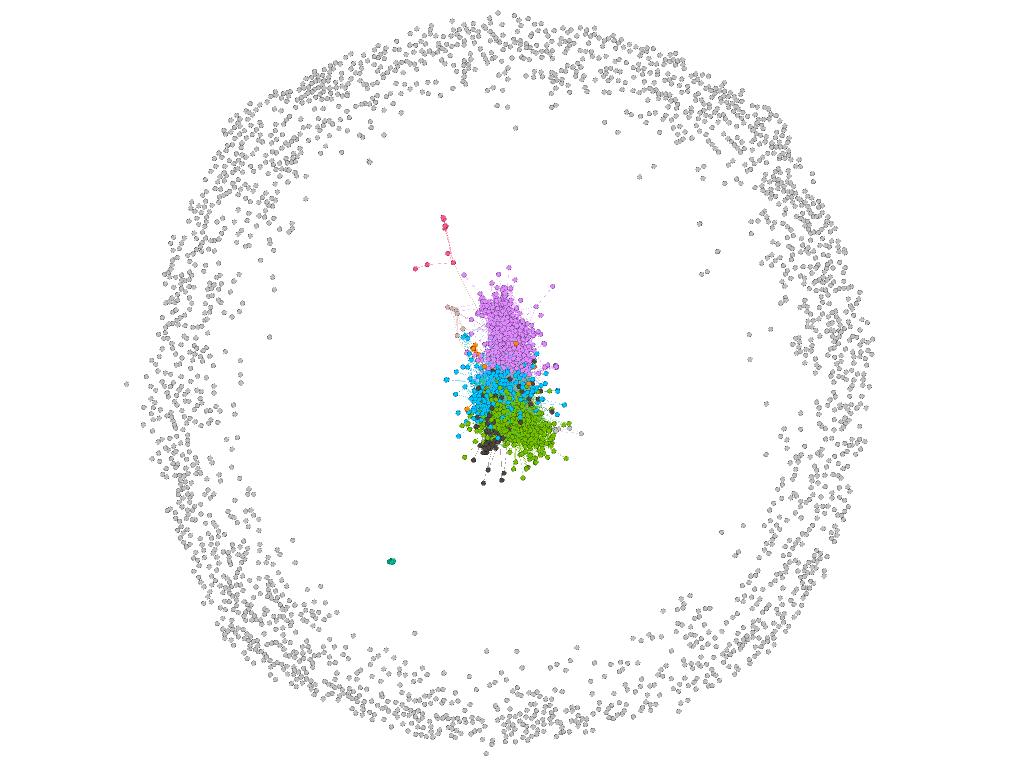
\includegraphics[width=\columnwidth]{graphics/atLeast10WorksCommunity.png}
	\caption{At least ten works in common graph coloured by community. Big cluster at the center, surrounded by loosely connected nodes.}
	\label{fig:graph10CommunityColoured}
	\end{center}
\end{figure}

Table~\ref{tab:graphComparision} shows some metrics about each graph. Requiring more works in common decreases average degree circumstantially but doesn't change a lot modularity or network diameter.

\begin{table}[!hbt]
	\begin{center}
	\caption{Graph analysis}
	\label{tab:graphComparision}
	\begin{tabular}{|l|c|c|c|}
		\hline
		Graph & Avg Degree & Graph Density & Modularity \\
		\hline
		One work in common & 267 & 0.09 & 0.2 \\
		\hline
		Ten works in common & 9 & 0.003 & 0.29 \\
		\hline
	\end{tabular}\\
	\smallskip
	\begin{tabular}{|l|c|c|}
		\hline
		Graph & Network Diameter & Connected Components \\
		\hline
		One work in common & 6 & 18 \\
		\hline
		Ten works in common & 7 & 2261 \\
		\hline
	\end{tabular}
	\end{center}
\end{table}

TODO ACOMODAR TODO ESTO, PRIMERO COSAS EN COMUN/ QUE QUIERO TENER LADO A LADO SOBRE ESTOS GRAFOS Y DESPUÉS PARTICULARIDADES, TOP10, UN POCO DE EXPLICACIÓN DE CADA UNO?

\begin{figure}[!hbt]
	\begin{center}
	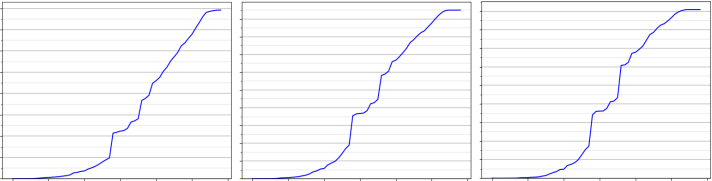
\includegraphics[width=\columnwidth]{graphics/edgesAccumulation.png}
	\caption{Grouwth of edges over time. For 1, 5 and 10 works in common graphs}
	\label{fig:accumulationEdges}
	\end{center}
\end{figure}

As proven by Fig.~\ref{fig:accumulationEdges} grouwth of edges by year follows the same distribution regardless of how many works in common are used to build the social network.
 
Fig.~\ref{fig:accumulationNodes} shows that more than half of the nodes are from last 18 years (2000 to 2018), giving us an idea of how much seiyuu industry is growing.

\begin{figure}[!hbt]
	\begin{center}
	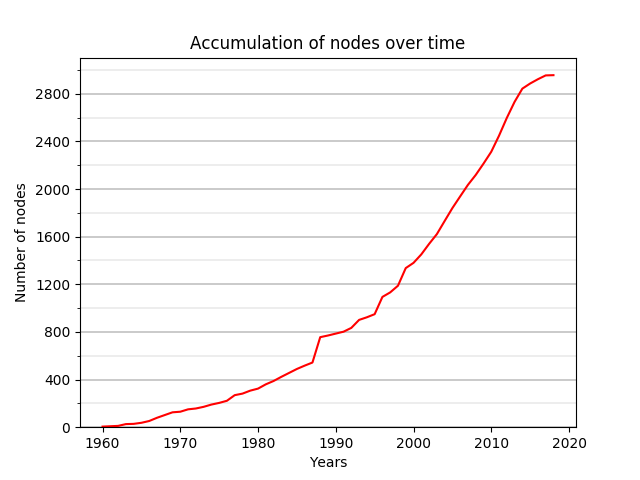
\includegraphics[width=\columnwidth]{graphics/nodesAccumulation.png}
	\caption{Grouwth of nodes over time.}
	\label{fig:accumulationNodes}
	\end{center}
\end{figure}

TODO HACER TOP 10 Y DEMÁS DATOS PARA CADA GRAFO (1 Y 10 TRABAJOS EN COMÚN) Y DIVIDIRLO EN SECCIONES, CAMBIAR LA EXPLICACIÓN DE MÁS ARRIBA TAMBIEN (AHORA YA NO NOS QUEDAMOS CON UNO SOLO PARA ESTA SECCIÓN, PERO SÍ PARA EL RESTO). PONER TAMBIÉN QUE ACÁ USO LAS DOS DEFINICIONES PARA MOSTRAR LO PARECIDAS QUE SON EN ESTRUCTURA Y QUE PARA EL RESTO USO LA DE AL MENOS 10 TRABAJOS

\subsection{At least 1 work in common}
\subsection{At least 10 works in common}

Tables~\ref{tab:top10Degree} and ~\ref{tab:top10BtwC} show top 10 nodes, for degree and betweenness centrality. 
\begin{table}[!hbt]
	\begin{center}
	\caption{Top 10 degree}
	\label{tab:top10Degree}
	\begin{tabular}{|l|c|}
		\hline
		Name & Degree\\ 
		\hline
		Takehito Koyasu & 311 \\ 
		\hline
		Akira Ishida & 273\\ 
		\hline
		Mamiko Noto & 258\\ 
		\hline
		Daisuke Namikawa & 232 \\ 
		\hline
		Katsuyuki Konishi & 229 \\ 
		\hline
		Keiji Fujiwara & 220 \\ 
		\hline
		Junichi Suwabe & 216 \\ 
		\hline
		Toshiyuki Morikawa & 215 \\ 
		\hline
		Rie Kugimiya & 213 \\ 
		\hline
		Nobuyuki Hiyama & 201 \\ 
		\hline
	\end{tabular}
	\end{center}
\end{table}

\begin{table}[!hbt]
	\begin{center}
	\caption{Top 10 Betweenness centrality}
	\label{tab:top10BtwC}
	\begin{tabular}{|l|c|}
		\hline
		Name & Betweenness Centrality \\ 
		\hline
		Takehito Koyasu & 18489.44 \\ 
		\hline
		Mamiko Noto & 10988.96 \\ 
		\hline
		Daisuke Namikawa & 9570.48 \\ 
		\hline
		Akira Ishida & 8299.19 \\ 
		\hline
		Rie Kugimiya & 7560.16 \\ 
		\hline
		Katsuyuki Konishi & 7413.71 \\ 
		\hline
		Kenichi Ogata & 7160.54 \\ 
		\hline
		Harumi Sakurai & 6775.76 \\ 
		\hline
		Keiji Fujiwara & 5980.58 \\ 
		\hline
		Yoshimasa Hosoya & 5607.95 \\ 
		\hline
	\end{tabular}
	\end{center}
\end{table}

